\documentclass{article}

\usepackage{fullpage}
\usepackage{amsfonts, amsmath}
\usepackage{url}
\usepackage{hyperref}
\usepackage[final]{pdfpages}

\pagenumbering{gobble}

\hypersetup{
    colorlinks=true,
    linkcolor=black
}

\begin{document}
\clearpage
\vspace*{\stretch{2}}
\begin{center}
\begin{minipage}{.6\textwidth}

\title{Automatic Music Generator \\ \vspace{2 pt} \Large{Project Proposal}}
\author{Sam Fleckenstein and Ross Nanopoulos}
\date{February 7, 2014}
\maketitle

\end{minipage}
\end{center}
\vspace{\stretch{3}}
\clearpage

\tableofcontents
\newpage

\section{Background}
Stuff goes here

\section{Intended Audience}
Stuff goes here

\section{Requirements}
\subsection{Song Parser}
Stuff goes here

\subsection{Learning Agent}
The job of the learning agent will be to take the raw music data gathered by the song parser and discover the relevant patterns in the music. There are a number of different algorithms that could be used to achieve this goal, but the current plan is to use a hidden Markov model to extract these patterns. This model was chosen because it can be used to represent processes where not all of the information about a state is know. This is useful because music is very complex and it is very difficult to determine every variable that goes into determining what should come next in a song. Another reason that hidden Markov models were chosen for this project is because they have been successfully applied the automatic generation of music.\\
\\
The learning agent is to be designed and implemented in such a way as to allow it to be easily swapped out for a different algorithm. This has several benefits. First, it will be easy to implement a completely different learning algorithm if one does not produce high enough quality results. Second, this will allow for easier testing of the various components of the project. It will be easy to set up dummy functions in the learning agent to accept data from the song parser in order to verify that the parsing is happening correctly. Dummy functions can also be used to pass specific patterns to the composition agent in order to verify that the patterns are applied correctly.

\subsection{Composition Agent}
alsdjkfhasdkhf

\section{Project Management}
\subsection{Communication}
In order to facilitate on-time delivery of the Intelligent Music Generator, in-person meetings will be held at least once at week on Thursdays at 4:30. In addition to this, meetings will be held as necessary to discuss upcoming deadlines as well as any issues that have come up. Communication will also happen during the rest of the week primarily via email.

\subsection{Work Division}
The primary responsibilities of each of the project members are as follows. Sam will be responsible for the primary development of the learning algorithms. Ross will be in charge of the implementation of the rest of the project. This is not a hard division of the work as each of the group members will also be working a great deal on the parts of the project they are not in charge of. This division of work fits well with the strengths and experience of each of the project members.

\section{Completed Work}
The work that is completed so far has been mostly research based. Various learning techniques for the learning agent have been examined before settling on using a Hidden Markov model. This model was chosen for several reasons. First, because it has been applied to various other projects with similar goals to this one. Second, because it appears to complex enough to produce interesting music, but simple enough that it will be possible to complete the project in the given timeline. In addition, pseudo-code has been written for the learning agent in order to more fully understand what will be required to implement the agent.

\section{Wishlist Features}
There are a number of features that will be included in the project if the required components are completed in time. First is some sort of user friendly UI. Currently, the only planned way of interacting with the program is through the command line. Since this method is not particularly user friendly, a UI with user controls may be added.\\
\\
Another feature that may be added is a different learning algorithm. If there is time, something like a neural network may be added to do the learning, instead of just using a hidden Markov model.\\
\\
A third feature that will be added if there is time is the ability to output the music to a Virtual Studio Technology. This would allow songs to be created that have more than one instrument. It would also allow the user or program to select what instrument they would like to use.

\nocite{*}

\bibliography{References}
\bibliographystyle{plain}

\newpage

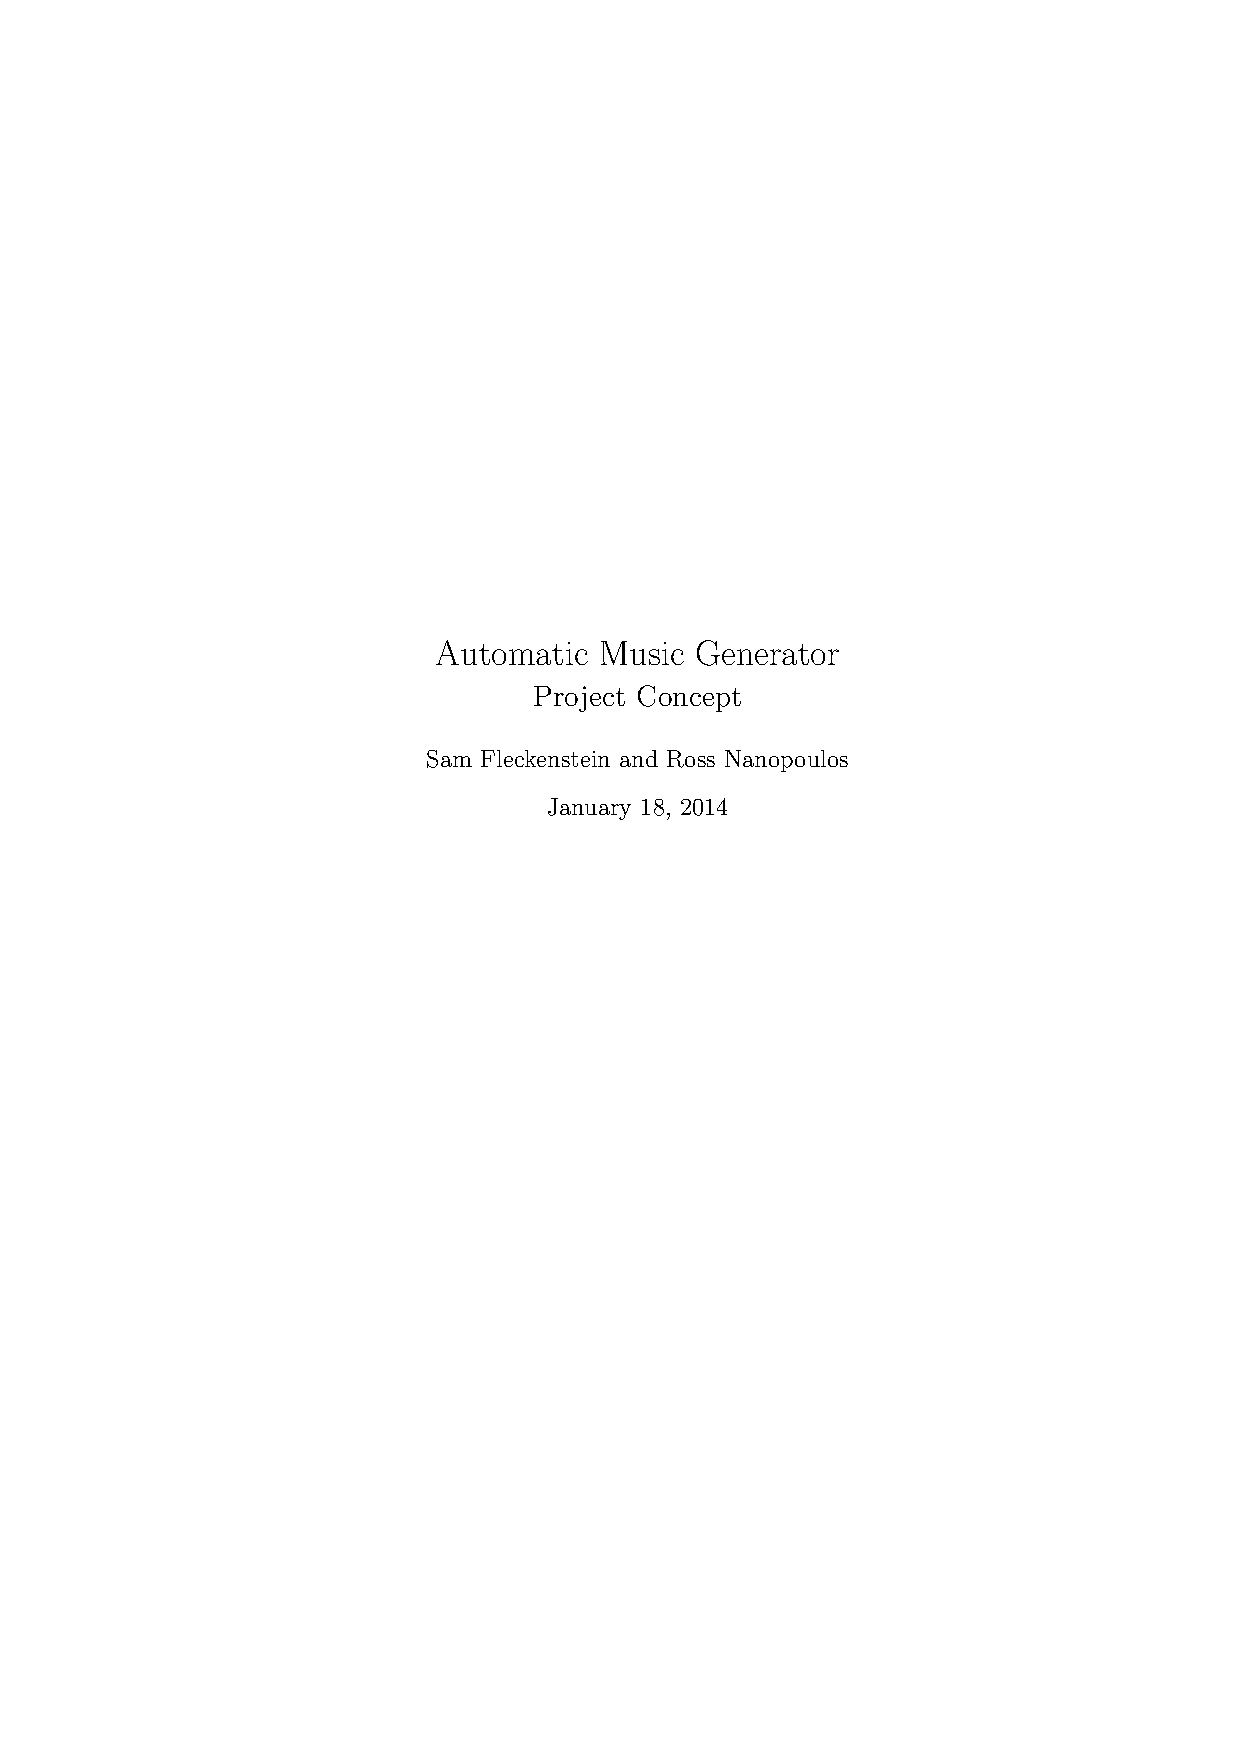
\includepdf[pages=-]{Concept.pdf}

\end{document}